\section{Optymalizator MySQL}

Zasadniczo każde zapytanie SQL skierowane do bazy danych MySQL może zostać zrealizowane na wiele różnych sposobów. Optymalizator jest częścią oprogramowania serwera MySQL, który odpowiada za wybranie najefektywniejszego sposobu wykonania zapytania (plan wykonania zapytania).
Proces ten ma kilka etapów. W pierwszej kolejności analizator MySQL dzieli zapytanie na tokeny i z nich tworzy drzewo (nazywane również \textit{drzewem analizy}). Na tym etapie przeprowadzana jest jednocześnie analiza składni zapytania. Następnym krokiem jest \textit{preprocessing}, w którego trakcie sprawdzane są między innymi: nazwy kolumn i tabel, a także nazwy i aliasy, aby zapewnić, że nazwy użyte w zapytaniu są np. jednoznaczne. Na kolejnym etapie weryfikowane są uprawnienia. Czynność ta może zajmować szczególnie dużo czasu, jeżeli serwer posiada bardzo dużą liczbę uprawnień. Po zakończeniu etapu \textit{preprocessingu} \textit{drzewo analizy} jest poprawne i gotowe do tego, aby optymalizator przekształcił je do postaci planu wykonania.

W MySQL stosowany jest optymalizator kosztowy. Oznacza to, że optymalizator szacuje koszt wykonania dla wariantów planu wykonania i wybiera ten z najmniejszym kosztem. Jednostką kosztu jest odczytanie pojedynczej, losowo wybranej strony danych o wielkości czterech kilobajtów. Wartość kosztu jest wyliczana na podstawie danych statystycznych, dlatego optymalizator wcale nie musi wybrać optymalnego planu.

Istnieją dwa rodzaje optymalizacji: \textit{statyczna} i \textit{dynamiczna}. Optymalizacja \textit{statyczna} przeprowadzana jest tylko raz i jest niezależna od wartości używanych w zapytaniu. W efekcie przeprowadzona raz będzie aktualna, nawet jeżeli zapytanie będzie wykonywane z różnymi wartościami. Natomiast optymalizacja dynamiczna bazuje na kontekście, w którym wykonywane jest zapytanie i jest przeprowadzana za każdym razem, kiedy polecenie jest wykonywane. Optymalizacja dynamiczna opiera się na wielu parametrach, takich jak: wartości w klauzuli WHERE czy liczba wierszy w indeksie, które znane są dopiero w momencie wykonania zapytania.

\subsection{Możliwości optymalizatora}
W tym podrozdziale przedstawiono kilka przykładowych optymalizacji, które może wykonać moduł serwer MySQL.

\begin{itemize}
	\item \textbf{Zmiana kolejności złączeń}. Podczas wykonywania zapytania tabele nie zawsze są łączone w takiej kolejności jak w zapytaniu. Zagadnienie jest dokładniej opisane w podrozdziale dotyczącym optymalizatora złączeń.
	\item \textbf{Zamiana OUTER JOIN na INNER JOIN.} Nawet jeżeli w zapytaniu użyjemy klauzuli OUTER JOIN, złączenie nie zawsze musi być wykonywany jako OUTER JOIN. Niektóre czynniki takie jak warunki w klauzuli WHERE czy schemat bazy danych mogą spowodować, że OUTER JOIN będzie równoznaczne złączeniu INNER JOIN. 
	\item \textbf{Przekształcenia algebraiczne.} Optymalizator przeprowadza transformacje algebraiczne takie jak: redukcja stałych, eliminowanie nieosiągalnych warunków czy stałych. Przykładowo warunek (2=2 AND a>2) może zostać przekształcony do postaci (a>2). Podobnie warunek (a<b AND b=c AND a=5) może być przekształcony do (b>5 AND b=c AND a=5).
	\item \textbf{Optymalizacja funkcji MIN(), MAX().}
	Serwer już na etapie optymalizacji zapytania może uznać wartości zwracane przez funkcje jako stałe dla reszty zapytania. W niektórych przypadkach optymalizator może nawet pominąć tabelę w planie wykonania zapytania, jeżeli jedyną wartością pobieraną z tabeli jest wynik funkcji MIN() lub MAX(). W takim przypadku w danych wyjściowych polecenia EXPLAIN znajdzie się ciąg tekstowy''Select tables optimized away''.
	Na rysunku ~\ref{fig:explain20} widzimy, że kolumna \textit{ref} dla pierwszego wiersza jest wartość ''const'', czyli najmniejsza wartość id z tabeli \textit{Users} została potraktowana jako stała.
	\begin{spverbatim}
		EXPLAIN SELECT * FROM Comments WHERE UserId = (SELECT MIN(id) FROM Users);
	\end{spverbatim}
\begin{figure}
	\centering
	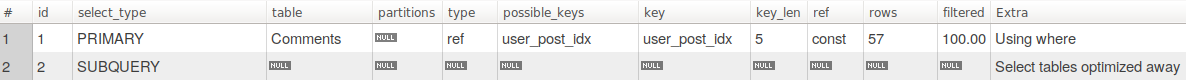
\includegraphics[scale = 0.37]{explain20.png}
	\label{fig:explain20}
\end{figure}
	\item \textbf{Optymalizacja funkcji COUNT().} Wyniki funkcji COUNT() bez klauzuli WHERE w niektórych silnikach (np. MyISM), również mogą zostać potraktowane jako stała, ale nie dotyczy to najpopularniejszego obecnie w MySQL silnika InnoDB.
	\textbf{Optymalizacja stałej tabeli}
	
	\item \textbf{Stałe tabele.} \textit{Stała tabela} jest to taka, która zawiera co najwyżej jeden wiersz lub warunek zawarty w klauzuli WHERE odnosi się do wszystkich kolumn klucza głównego, albo do indeksu UNIQUE NOT NULL. W takim przypadku MySQL może zwrócić wartość jeszcze przed wykonaniem zapytania i potraktować jako stałą dla dalszej części zapytania.
\end{itemize}

\subsection{Dane statystyczne dla optymalizatora}
Przechowywaniem danych statystycznych jest zadaniem silników bazy danych. Z tego powodu w zależności od użytego silnika przechowywane wartości statystyczne mogą być różne. Przykładowo silnik MyISM przechowuje informacje o aktualnej liczbie rekordów w tabeli, a InnoDB takiej informacji nie przechowuje, natomiast niektóre silniki, np. Archive, wcale nie przechowują danych statystycznych.

\subsection{Plan wykonania zapytania}
Wynikiem optymalizacji jest plan wykonania zapytania. Jest on zapisywany w postaci drzewa instrukcji, które kolejno wykonywane doprowadzą do zwrócenia wyniku.
\begin{spverbatim}
	SELECT * FROM Posts p LEFT JOIN PostTypes pt ON p.PostTypeId = pt.Id LEFT JOIN PostLinks pl ON p.Id = pl.PostId LEFT JOIN LinkTypes lt on pl.LinkTypeId = lt.id WHERE PostID = 9;
\end{spverbatim}
Sposób łączenia tabel moglibyśmy przedstawić jak na poniższym schemacie.
 \begin{center}
 	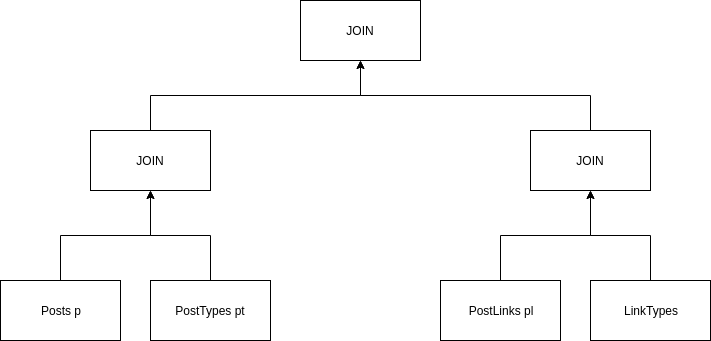
\includegraphics[scale =0.45]{PLAN_WYKONANIA_1.png} 
 \end{center}
W rzeczywistości drzewo instrukcji przybiera postać drzewa lewostronnie zagnieżdżonego. Cechą charakterystyczną tych drzew jest to, że sekwencje operacji łączenia są wykonywane w sposób potokowy. Przykład takiego drzewa jest przedstawiony na poniższym rysunku.
\begin{center}
	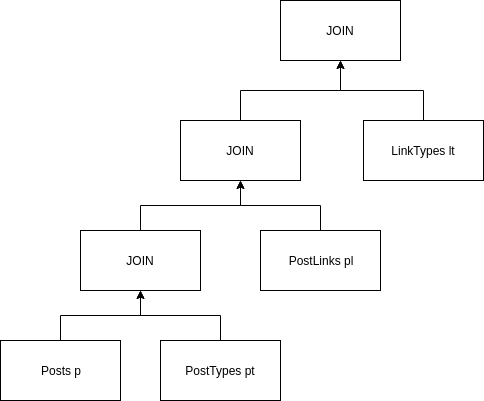
\includegraphics[scale =0.45]{PLAN_WYKONANIA_2.png} 
\end{center}
Analizując wyniki polecenia EXPLAIN dla powyższego zapytania, używając aplikacji \textit{MySQL Workbench} możliwe jest wyświetlenie graficznej postaci odpowiadającej drzewu instrukcji.
\begin{center}
	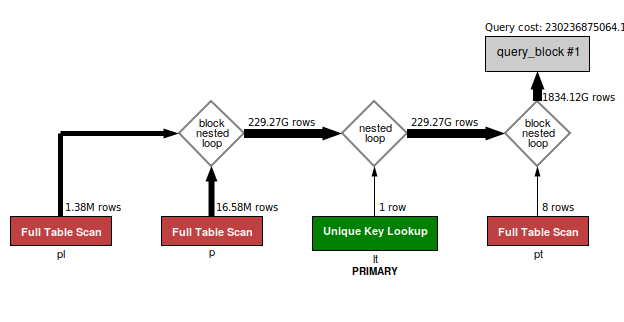
\includegraphics[scale =0.5]{explain21.png} 
\end{center}
Drzewo otrzymane jako wynik polecenia EXPLAIN jest drzewem lewostronnie zagnieżdżonym. Zauważamy też, że optymalizator zdecydował się zamienić kolejność złączeń, aby zminimalizować koszt wykonania zapytania.

\subsection{Optymalizator złączeń}
Większość operacji złączeń można wykonać na różne sposoby, uzyskując ten sam wynik. Zamiana kolejności jest bardzo skuteczną formą optymalizacji zapytań. W tym podrozdziale rozważono następujące zapytanie.
\newpage
\begin{spverbatim}
	SELECT u.Id, p.Id, c.Id, pt.`Type` FROM Users u INNER JOIN Posts p ON u.Id = p.OwnerUserId  INNER JOIN Comments c ON c.UserId = u.Id INNER JOIN 
	PostTypes pt ON pt.Id = p.PostTypeId WHERE u.Id = 4;
\end{spverbatim}
\bigskip
Wykonując polecenie z prefiksem EXPLAIN, otrzymano następujący wynik:
\begin{center}
	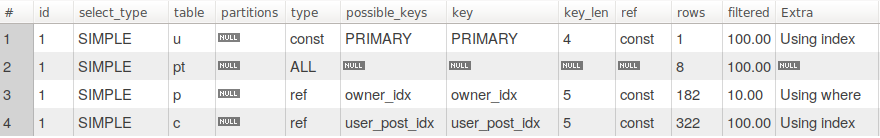
\includegraphics[scale =0.45]{explain22.png} 
\end{center}
Następnie zmodyfikowano zapytanie dodając słowo kluczowe STRAIGHT\textunderscore JOIN, aby wymusić kolejność złączeń taką jak w zapytaniu.
\begin{center}
	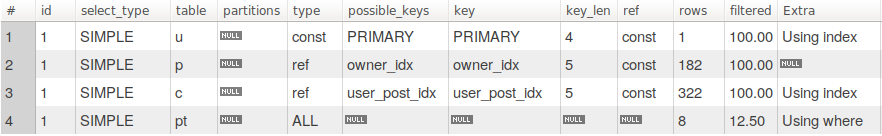
\includegraphics[scale =0.45]{explain23.png} 
\end{center}
Wyniki polecenia są niemalże identyczne, jedyną różnicą jest kolejność dokonywanych złączeń. Koszt ostatniego zapytania można sprawdzić wykonując następujące polecenie:
\begin{spverbatim}
	SHOW STATUS LIKE 'Last_Query_Cost';
\end{spverbatim}
Koszt pierwszego zapytania, którego kolejność została zamieniona na etapie optymalizacji, wynosi 6510. Koszt drugiego zapytania wynosi 66868! Zamiana kolejności złączeń zmniejszyła koszt dziesięciokrotnie.
W kolejnym kroku włączono profilowanie zapytań za pomocą komendy:
\begin{spverbatim}
	SET PROFILING = 1;
\end{spverbatim}
\bigskip
Wykonano 10 zapytań dla każdego wariantu i policzono średni czas, jaki serwer MySQL spędzał na etapie ''executing'', czyli etapie faktycznego wykonywania zapytania. Dla zapytania z kolejnością wybraną przez optymalizator średnia wartość wyniosła 0.04 sekundy, natomiast przy wymuszonej kolejności łączeń w zapytaniu wartość ta wyniosła 0.28 sekundy. 

Powyższy eksperyment pokazuje, że zamiana kolejności złączeń jest bardzo skuteczną formą optymalizacji i może prowadzić do wielokrotnego zmniejszenia kosztu zapytania. Oczywiście nadal może się zdarzyć sytuacja, kiedy zapytanie z wymuszoną kolejnością załączeń będzie wydajniejsze, ponieważ optymalizator MySQL nie zawsze może sprawdzić wszystkie potencjalne kombinacje złączeń, ale w zdecydowanej większości przypadków optymalizator złączeń okazuje się skuteczniejszy od człowieka.

\subsection{Konfiguracja optymalizatora złączeń}
Optymalizator złączeń stara się wygenerować plan zapytań o najniższym możliwym koszcie. W idealnym przypadku optymalizator zweryfikowałby wszystkie możliwe kombinacje złączeń. Niestety operacja łączenia dla \textit{n} tabel będzie miała \textit{n!} możliwych kombinacji. Oznacza to, że dla dziesięciu tabel złączenia mogą zostać przeprowadzone na 3628800 różnych sposobów i gdyby optymalizator zdecydował się przetestować każdy dostępny scenariusz, kompilacja mogłaby zająć wiele godzin, a nawet dni. Do określenia, jak wiele planów powinien przetestować optymalizator służy opcja \textit{optimizer\textunderscore search\textunderscore depth}. Na ogół im niższa wartość zmiennej, tym szybciej optymalizator zwróci plan wykonania, ale zmniejsza się też prawdopodobieństwo optymalności planu. Wartość 0 oznacza, że MySQL dla każdego zapytania dobierze odpowiednią (zdaniem optymalizatora) przestrzeń przeszukiwania.

Aby pokazać wpływ parametru \textit{optimizer\textunderscore search\textunderscore depth} przygotowano następujący kod SQL, który tworzy dwie tabele, a następnie wypełnia je losowymi danymi.

\begin{spverbatim}
	CREATE TABLE `lecturers`
	(
	`id` INT(11) NOT NULL AUTO_INCREMENT,
	PRIMARY KEY (`id`)
	);
	CREATE TABLE `students`
	(
	`id` INT(11) NOT NULL AUTO_INCREMENT,
	`lecturer_id` INT(11) NOT NULL,
	`value` SMALLINT(6) NOT NULL,
	PRIMARY KEY (`id`),
	INDEX `lecturer_id` (`lecturer_id`),
	INDEX `value` (`value`)
	);
	INSERT INTO `lecturers` VALUES (1), (2);
	
	DELIMITER ;;
	CREATE PROCEDURE fill_tables()
	BEGIN
		DECLARE i INT DEFAULT 0;
		WHILE i <= 1000 DO
			INSERT INTO `students` (`id`, `lecturer_id`, `value`) VALUES (0, 1, i);
			INSERT INTO `students` (`id`, `lecturer_id`, `value`) VALUES (0, 2, i);
			SET i = i + 1;
		END WHILE;
	END;;
	DELIMITER ;
	
	CALL fill_tables();
\end{spverbatim}
\bigskip
W kolejnym kroku wykonano wielokrotnie następujące zapytanie:
\bigskip
\begin{spverbatim}
	SELECT COUNT(*) FROM table_parent AS p WHERE 1
	AND EXISTS (SELECT 1 FROM students AS s WHERE s.lecturer_id = p.id AND s.value = 1 LIMIT 1)
	AND EXISTS (SELECT 1 FROM students AS s WHERE s.lecturer_id = p.id AND s.value = 2 LIMIT 1)
	AND EXISTS (SELECT 1 FROM students AS s WHERE s.lecturer_id = p.id AND s.value = 3 LIMIT 1)
	AND EXISTS (SELECT 1 FROM students AS s WHERE s.lecturer_id = p.id AND s.value = 4 LIMIT 1)
	AND EXISTS (SELECT 1 FROM students AS s WHERE s.lecturer_id = p.id AND s.value = 5 LIMIT 1)
	AND EXISTS (SELECT 1 FROM students AS s WHERE s.lecturer_id = p.id AND s.value = 6 LIMIT 1)
	AND EXISTS (SELECT 1 FROM students AS s WHERE s.lecturer_id = p.id AND s.value = 7 LIMIT 1)
	AND EXISTS (SELECT 1 FROM students AS s WHERE s.lecturer_id = p.id AND s.value = 8 LIMIT 1)
	AND EXISTS (SELECT 1 FROM students AS s WHERE s.lecturer_id = p.id AND s.value = 9 LIMIT 1)
	AND EXISTS (SELECT 1 FROM students AS s WHERE s.lecturer_id = p.id AND s.value = 10 LIMIT 1)
\end{spverbatim}
Zmieniając parametr \textit{optimizer\textunderscore search\textunderscore depth}, dla każdej wartości zmiennej zapisano średni czas wykonania polecenia EXPLAIN. Wyniki zamieszczono w poniższej tabeli.

\begin{center}
	\begin{tabular}{ |c|c| } 
		\hline
		optimizer\textunderscore search\textunderscore depth & czas [sekund]\\ 
		\hline
		0 & 1.8\\
		1 & 0.0011\\
		2 & 0.0019\\
		3 & 0.0059\\
		5 & 0.6\\
		10 & 15\\
		20 & 22\\
		30 & 27\\
		62 & 36\\
		\hline
	\end{tabular}
\end{center}
Wraz ze wzrostem wartości parametru wzrastał czas wykonywania polecenia SQL. W kolejnym kroku włączono profilowania i sprawdzono, na który z etapów serwer spędził najwięcej czasu. Wyniki posortowano według czasu. Na poniższym zrzucie ekranu umieszczono profil zapytania dla wartości 62.
\begin{center}
	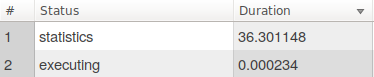
\includegraphics[scale =0.60]{profile1.png} 
\end{center}
Profilowanie zapytania wskazuje, że przez większość czasu zapytania, serwer zbierał dane, które pozwolą mu wybrać optymalny plan wykonania zapytania. Okazało się, że dla pewnych zapytań, próba wybrania optymalnego rozwiązania może skończyć się gigantycznym wydłużeniem czasu zapytania. Co ciekawe nawet dla wartości 0 optymalizacja okazał się nieefektywna, co prowadzi do wniosku, że czasami jedym rozwiązaniem w przypadku, kiedy serwer zbyt dużą ilość czasu spędza na szukaniu optymalnego planu, jest ręczna zmiana wartości parametru \textit{optimizer\textunderscore search\textunderscore depth}.

Drugim atrybutem, który służy do konfiguracji optymalizatora złączeń jest \textit{optimizer\textunderscore prune\textunderscore level}. Parametr decyduje o tym, czy optymalizator może wykorzystać heurystyki do wybrania optymalnego planu. Jeżeli ta opcja zostanie włączona, optymalizator może pominąć niektóre plany, bazując na pewnych heurystykach. Dokumentacja MySQL wskazuje, że relatywnie rzadko dochodzi do sytuacji, kiedy optymalizator pomija optymalny plan wykonania, a włączenie tej opcji może znacznie przyśpieszyć proces optymalizacji. Dlatego też domyślną wartością jest 1, co oznacza, że serwer może bazować na heurystykach.

Aby pokazać wpływ parametru na wydajność zapytania, wykorzystano jeszcze raz zapytanie do wygenerowanej tabeli \textit{Students}. Najpierw ustawiono wartość parametru optimizer\textunderscore search\textunderscore depth=0, a następnie optimizer\textunderscore prune\textunderscore level=0. Poprzedni eksperyment pokazuje, że to zapytanie powinno wykonać się w czasie mniej więcej 1.8 sekundy, ale tym razem wymagało średnio ok. 3.8 sekundy, czyli ponad 2 dłużej. Następnie ustawiono wartość optimizer\textunderscore search\textunderscore depth=62 i ponownie zmierzono średni czas wykonania zapytania. Tym razem zapytanie trwało średnio 121 sekund, co oznacza prawie czterokrotny spadek wydajności w stosunku do \textit{optimizer\textunderscore prune\textunderscore level}=1. Dlatego zalecane jest pozostawienie domyślnej wartości \textit{ optimizer\textunderscore prune}, chyba że mamy pewności pominięcia optymalnego planu zapytania.

\subsection{Konfiguracja statystyk tabel InnoDB}
Dla tabeli InnoDB zbierane są dwa rodzaje statystyk: trwałe i nietrwałe. Trwałe zapisywane są na dysku twardym i przechowywane są pomiędzy restartami serwera, nietrwałe (ulotne) są usuwane po każdym restarcie. 

\subsubsection{Trwałe statystyki}
Od wersji MySQL 5.6.6 trwałe statystyki są domyślnie włączone dla wszystkich tabel InnoDB, ale można je wyłączyć dla wszystkich tabel poprzez ustawienie parametru \textit{innodb\textunderscore stats\textunderscore persistent} = OFF, lub poprzez ustawienie \textit{stats\textunderscore persistent} = 0 dla wybranej tabeli.

\paragraph{Konfiguracja automatycznego przeliczania statystyk}\mbox{}\\
\smallskip
Standardowo przeliczenie trwałych statystyk dla tabeli ma miejsce, jeżeli zmodyfikowane zostanie więcej niż 10 \% wierszy w tabeli. Jeżeli chcemy wyłączyć automatyczne kalkulowanie, należy ustawić parametr \textit{innodb\textunderscore stats\textunderscore auto\textunderscore recalc} = false. Należy pamiętać o tym, że przeliczanie statystyk odbywa się asynchronicznie, to znaczy serwer nie wykonuje kalkulacji natychmiastowo po zmodyfikowaniu 10 \% wierszy, ale próbuje znaleźć optymalny czas. Jeżeli chcemy wymusić przeliczenie wywołujemy polecenie ANALYZE TABLE. Jeżeli dodajemy indeks do tabeli lub kolumna jest usuwana, przeliczenie odbywa się automatycznie.

\paragraph{Obliczanie statystyk}\mbox{}\\
Dane statystyczne dotyczące tabeli są obliczane na podstawie pewnej grupy losowo wybranych wierszy. Domyślnie skanowane jest 20 stron, ale wartość ta może być zmieniona dla konkretnej tabeli poprzez parametr \textit{innodb\textunderscore stats\textunderscore persistent\textunderscore sample\textunderscore pages} lub parametr \textit{stats\textunderscore sample\textunderscore pages}. Zmianę wartości parametru powinna zostać rozpatrzona w następujących przypadkach:
\begin{itemize}
	\item \textbf{Wartości statystyczne odbiegają od rzeczywistych.} \linebreak
	Aby sprawdzić dokładność statystyk dla wybranego indeksu możemy porównać dane statystyczne znajdujące się w tabeli \textit{innodb\textunderscore index\textunderscore stats} i porównać z liczbą rzeczywistych unikatowych wartości indeksu.
	
	Sprawdzono dokładność danych statystycznych dla indeksów tabeli \textit{Posts} i różnych liczb skanowanych stron. Tabela \textit{Posts} zawiera dwa indeksy: owner\textunderscore idx (owner\textunderscore id) oraz favorite\textunderscore idx (FavoriteCount, Score).
	W tym celu przygotowano cztery zapytania.
	Dwa dla owner\textunderscore idx:
	\begin{spverbatim}
		SELECT COUNT(DISTINCT OwnerUserId) FROM Posts; #liczba unikalnych
		wartości indeksu
		SELECT stat_value FROM mysql.innodb_index_stats WHERE 
		database_name= 'stackOverflowMedium' AND table_name = 'Posts' 
		AND index_name = 'owner_idx' 
		AND	stat_name = 'n_diff_pfx01';
	\end{spverbatim}
	Oraz dwa dla favorite\textunderscore idx:
	\begin{spverbatim}
		SELECT COUNT(DISTINCT FavoriteCount, Score) FROM Posts;
		SELECT stat_value FROM mysql.innodb_index_stats WHERE 
		database_name= 'stackOverflowMedium' AND table_name = 'Posts' 
		AND index_name = 'favorite_idx' 
		AND	stat_name = 'n_diff_pfx01';
	\end{spverbatim}
	W poniższej tabeli zamieszczono wyniki eksperymentu.
	\begin{center}
		\begin{tabular}{ |c|c|c|c| } 
			\hline
			sample pages & owner\textunderscore idx & favorite\textunderscore idx & ANALYZE TABLE czas [s]\\ 
			\hline
			1 & 3597380 & 8368 & 0.04\\
			20 & 1364542 & 159689 & 0.06\\
			400 & 1443184 & 22930 & 0.4\\
			8000 & 1435072 & 23311 & 4.3\\
			16000 & 1435072 & 23311 & 7\\
			\hline
			rzeczywista wartość & 1435072 & 23311 & \\
			\hline
		\end{tabular}
	\end{center}
	Wraz ze wzrostem liczby stron użytych do analizy wzrasta dokładność statystyk, ale rośnie czas przeprowadzania analizy tabeli. Dla domyślnej wartości parametru, oszacowana wartość unikatowych wartości indeksu favorite\textunderscore idx diametralnie różni się od rzeczywistej, co może doprowadzić do wyboru nieoptymalnego indeksu na etapie optymalizacji. W takiej sytuacji dobrym wyborem będzie zwiększenie wartości parametru.
	
	\item \textbf{Zbyt długi czas zbierania statystyk dla tabeli} \linebreak
	Analizując wyniki tabeli można stwierdzić, że przy wysokich wartościach parametru, serwer MySQL spędza dużo czasu na obliczaniu statystyk dla tabeli, co może prowadzić, szczególnie przy często zmieniających się tabelach, do wysokiego wykorzystania zasobów, szczególnie operacji odczytów z dysku.
\end{itemize}

\subsection{Podsumowanie}
W tym rozdziale przedstawiono ogólne zasady działania optymalizatora MySQL. Zwrócono uwagę przede wszystim na to, że optymalizator bazuje jedynie na danych statystycznych oraz pewnych heurystykach, stąd decyzje podejmowane przez niego nie muszą być optymalne. W skrajnych przypadkach optymalizator może nawet znacząco pogorszyć wydajność zapytań, dlatego ważna jest świadomość jego ograniczeń oraz umiejętność poprawnego dostrajania jego parametrów.

